\documentclass[12pt]{article}

\usepackage{eucal}
\usepackage{graphicx}
\usepackage{enumerate}
\usepackage[utf8]{inputenc}
\usepackage{amsmath}

\begin{document}

\begin{sffamily}
\begin{Large}
\noindent
\centering \textbf{Technical notes on Angular Correlation Analysis}\\
\vspace{1cm}
\end{Large}
\end{sffamily}
\noindent
Written by Jonas A. Sellberg on 2013-07-06.\\

\vspace{1cm}
\begin{sffamily}
\begin{Large}
\textbf{Correlation Algorithms}\\
\end{Large}
\end{sffamily}
\vspace{0.3cm}

Several correlation algorithms have been proposed for coherent x-ray scattering (CXS) and this technical note, I will attempt to summarize them and pinpoint important technical differences between them. Among the most widely used expressions we find intensity-based correlations
\begin{equation}\label{xcca-int}
C_{q_1,q_2}(\Delta) = \frac{\left\langle I(q_1,\varphi)\cdot I(q_2,\varphi+\Delta)\right\rangle_{\varphi}-\left\langle I(q_1,\varphi)\right\rangle_{\varphi}\left\langle I(q_2,\varphi)\right\rangle_{\varphi}}{\left\langle I(q_1,\varphi)\right\rangle_{\varphi}\cdot\left\langle I(q_2,\varphi)\right\rangle_{\varphi}},
\end{equation}
where $I(q_1,\varphi)$ is the instantaneously scattered intensity at momentum transfer magnitude $q_1$ and azimuthal angle $\varphi$, $\Delta$ is the angular shift between $I(q_1,\varphi)$ and $I(q_2,\varphi+\Delta)$, and $\left\langle I(q,\varphi) \right\rangle_{\varphi} = \frac{1}{2\pi} \int_0^{2\pi} I(q,\varphi) d\varphi = I(q)$ denotes the angular average. Mathematically, if one uses the fact that the intensity $I(q,\varphi)$ is a $2\pi$-periodic function of $\varphi$, Eq. (\ref{xcca-int}) can be shown to be equivalent to
\begin{equation}\label{xcca-fluct}
C_{q_1,q_2}(\Delta) = \frac{\left\langle \left(I(q_1,\varphi)-\left\langle I(q_1,\varphi)\right\rangle_{\varphi}\right)\cdot\left(I(q_2,\varphi+\Delta)-\left\langle I(q_2,\varphi)\right\rangle_{\varphi}\right)\right\rangle_{\varphi}}{\left\langle I(q_1,\varphi)\right\rangle_{\varphi}\cdot\left\langle I(q_2,\varphi)\right\rangle_{\varphi}}.
\end{equation}
Eq. (\ref{xcca-fluct}) is in contrast to Eq. (\ref{xcca-int}) based on correlations between fluctuations of intensities around the mean intensity $I(q)$ over all angles $\varphi$.  However, as we shall see in the next paragraph, there are some technical differences between the two expressions.
%For the discussion below, we will assume that $q_1 = q_2 = q$, which reduces the correlation function $C_{q_1,q_2}(\Delta) = C_{q}(\Delta)$ to 2 dimensions, but the conclusions can be shown to be true for the general 3-dimensional correlation function $C_{q_1,q_2}(\Delta)$.

\newpage

\vspace{1cm}
\begin{sffamily}
\begin{Large}
\textbf{Gaps}\\
\end{Large}
\end{sffamily}
\vspace{0.3cm}

Suppose now that the detector that samples the coherently scattered intensity lacks part of the solid angle at a given momentum transfer magnitude $q$ of interest, so that $I(q,\varphi)$ is only partly sampled and cannot be determined for all $\varphi$ in the interval $[0,2\pi)$ of interest. Furthermore, the detector pixels are of finite size, which corresponds to some angular segment $d\varphi = 2\pi/N_{\varphi}$, which means the angular average turns into an angular sum
\begin{equation}\label{discete-avg}
\left\langle I(q,\varphi) \right\rangle_{\varphi} = \frac{1}{N_{\varphi}} \sum_{i=0}^{N_{\varphi}} I(q,\varphi_i),
\end{equation}
where $N_{\varphi}$ is the number of angular bins at momentum transfer magnitude $q$. The partial sampling at $q$ leaves us two choices to compute Eq. (\ref{discete-avg}):\\

A. We can include the gaps in the detector so that the angular bins span the whole interval $[0,2\pi)$ but the intensities where the gaps are present has to be determined artificially by putting them to 0, the mean of the rest of the pixels, or by interpolation.

B. We can exclude the gaps in the detector so that the angular bins no longer span the whole interval $[0,2\pi)$ and consequently $N_{\varphi}$ is lowered and depends on what function the sum is performed over.\\

If no external knowledge of the angular dependence of the intensity is available, one may want to avoid interpolation over larger gaps, and we shall therefore set the intensities inside the gaps to 0 when we include the gaps, which corresponds to the mean if Eq. (\ref{xcca-fluct}) is used. We can now test how the modification of the scattered intensity due to the presence of the gaps will alter the correlation function $C(\Delta)$ at a given $q$. For simplicity, we assume $q_1 = q_2 = q$ and that the angular dependence of the scattered intensity is a simple sine function with a period of $2\pi/3$ that has an amplitude of 1 centered around a mean of 3 (see Fig. \ref{fig-include-gaps}, top). We now introduce arbitrary gaps in the sampling of the true signal, which results in a gap-modified signal where the absence of information about the scattered intensity is replaced by zeros (see Fig. \ref{fig-include-gaps}, middle). $C(\Delta)$) is then calculated for the true signal using Eq. (\ref{xcca-int}) (the result is equivalent using Eq. (\ref{xcca-fluct}), see Fig. \ref{fig-exclude-gaps}, bottom) and the gap-modified signal using Eq. (\ref{xcca-int}) and Eq. (\ref{xcca-fluct}) and is presented in Fig. \ref{fig-include-gaps}, bottom. The correlation function of the true signal shows a clear 3-folded symmetry, which is indicative of the symmetry of the scattered intensity, and this is very much captured by $C(\Delta)$ calculated from the gap-modified signal using Eq. (\ref{xcca-fluct}), although the amplitude is slightly modified due to the presence of the gaps. If we calculate $C(\Delta)$ from the gap-modified signal using Eq. (\ref{xcca-int}), the signal is severely altered and the 3-folded symmetry is no longer captured. This can be attributed to the correlations of the gaps themselves, which in this case are dominated by a 2-folded symmetry, and since the fluctuations between gaps (i.e. zeros) and signal are stronger than the fluctuations in the signal itself they will dominate $C(\Delta)$. The same will be true when we calculate $C(\Delta)$ using Eq. (\ref{xcca-fluct}), but then the zeros of the gaps correspond roughly to the mean of the fluctuations that we correlate (there is a slight shift in the calculated mean from the true mean due to the gaps) and hence the fluctuations in the scattered intensity will still dominate $C(\Delta)$.

\begin{figure}
  \centering
  \scalebox{0.7}{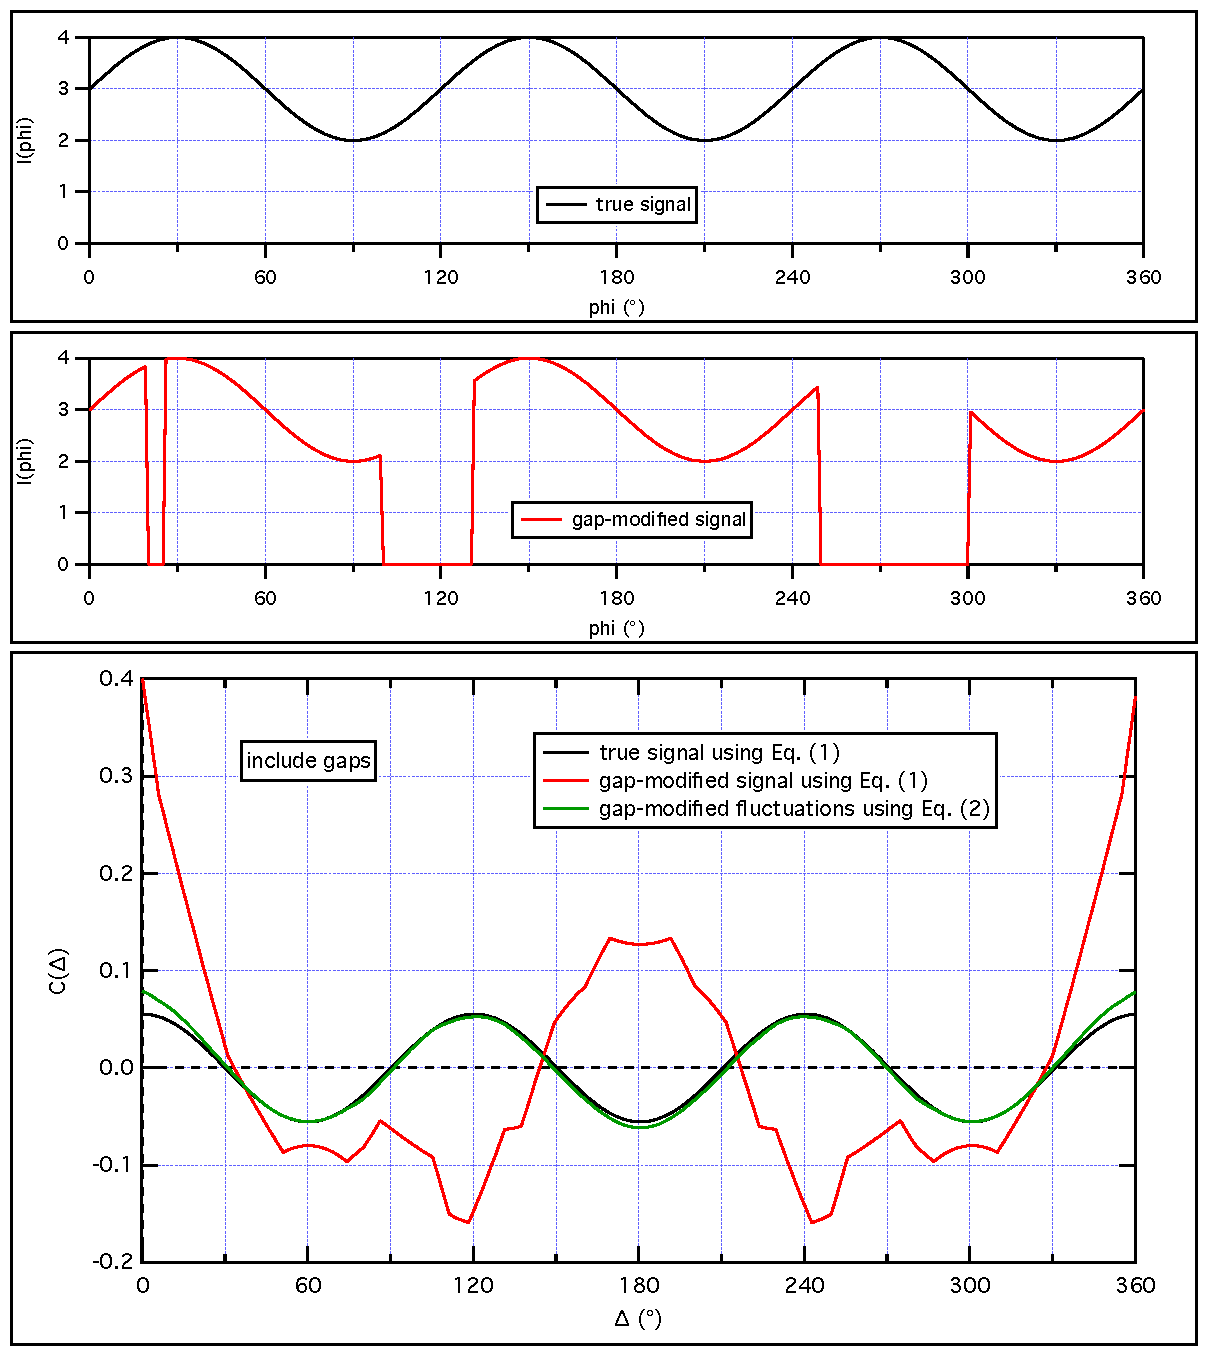
\includegraphics{./Layout0-include_gaps.pdf}}
  \caption{ \small (TOP) Model signal of the scattered intensity at arbitrary $q$ with an angular dependence of sine function with a period of $2\pi/3$ that has an amplitude of 1 centered around a mean of 3. (MIDDLE) Gap-modified signal where the presence of arbitrarily placed gaps modify the angular dependence of the scattered intensity by replacing the true signal by zeros. (BOTTOM) $C(\Delta)$ from correlating while including the gaps for the true signal using Eq. (\ref{xcca-int}) (black curve), the gap-modified signal using Eq. (\ref{xcca-int}) (red curve), and the gap-modified fluctuations using Eq. (\ref{xcca-fluct}) (green curve).}
  \label{fig-include-gaps}
\end{figure}

\newpage
If we instead exclude the gaps, we won't need to approximate the scattered intensity in the gaps, but $N_{\varphi}$ will in turn be altered. If (B) is used with Eq. (\ref{xcca-int}) we now obtain
\begin{align}\label{discrete-int}
C_{q_1,q_2}(\Delta) = \frac{1}{\sum_{i=0}^{N_1} I(q_1,\varphi_i)\cdot\sum_{i=0}^{N_2} I(q_2,\varphi_i)} \\
\cdot\left(\sum_{i=0}^{N(\Delta)} I(q_1,\varphi_i)\cdot I(q_2,\varphi_i+\Delta)-\sum_{i=0}^{N_1} I(q_1,\varphi_i)\cdot\sum_{i=0}^{N_2} I(q_2,\varphi_i)\right).\nonumber
\end{align}
If (B) is used with Eq. (\ref{xcca-fluct}) we instead obtain
\begin{align}\label{discrete-fluct}
C_{q_1,q_2}(\Delta) = \frac{1}{\sum_{i=0}^{N_1} I(q_1,\varphi_i)\cdot\sum_{i=0}^{N_2} I(q_2,\varphi_i)} \\
\cdot\left(\sum_{i=0}^{N(\Delta)} I(q_1,\varphi_i)\cdot I(q_2,\varphi_i+\Delta)+\sum_{i=0}^{N_1} I(q_1,\varphi_i)\cdot\sum_{i=0}^{N_2} I(q_2,\varphi_i)\right) \nonumber \\
-\frac{1}{\sum_{i=0}^{N_1} I(q_1,\varphi_i)\cdot\sum_{i=0}^{N_2} I(q_2,\varphi_i)} \nonumber \\
\cdot\left(\sum_{i=0}^{N_1} I(q_1,\varphi_i)\cdot\sum_{i=0}^{N(\Delta)} I(q_2,\varphi_i)+\sum_{i=0}^{N(\Delta)} I(q_1,\varphi_i)\cdot\sum_{i=0}^{N_2} I(q_2,\varphi_i)\right).\nonumber
\end{align}
The denominator is the same in both Eq. (\ref{discrete-int}) and Eq. (\ref{discrete-fluct}), but we see that there is a difference between the nominator terms. The first term in the nominator, which corresponds to the correlation between the intensities, is in both cases a sum over $N(\Delta)$ and thus the same. The second term has also the same summation indices but opposite sign, and has to be counteracted by the third and fourth term. This yields that for Eq. (\ref{xcca-int}) to be equal to Eq. (\ref{xcca-fluct}), we must have
\begin{align}\label{discrete-int=fluct}
2\sum_{i=0}^{N_1} I(q_1,\varphi_i)\cdot\sum_{i=0}^{N_2} I(q_2,\varphi_i) = \\
= \sum_{i=0}^{N_1} I(q_1,\varphi_i)\cdot\sum_{i=0}^{N(\Delta)} I(q_2,\varphi_i)+\sum_{i=0}^{N(\Delta)} I(q_1,\varphi_i)\cdot\sum_{i=0}^{N_2} I(q_2,\varphi_i). \nonumber
\end{align}
This is by no means true in general, since $N(\Delta)$ is a function of the angular shift and thus depends on $\Delta$ whereas $N_1$ and $N_2$ does not.

We can once again test the effect of the gaps on $C(\Delta)$ when we instead exclude the gaps. In the bottom section of Fig. \ref{fig-exclude-gaps} we see that when we use Eq. (\ref{xcca-int}) to calculate $C(\Delta)$ (i.e. correlate the intensities), the signal is severely distorted and the 3-folded symmetry is lost. When we use Eq. (\ref{xcca-fluct}) to calculate $C(\Delta)$ (i.e. correlate the fluctuations), on the other hand, the 3-folded symmetry persists despite the gaps in the sampling of the scattered intensity. This means that the angular shift-dependence of the number of angular bins $N(\Delta)$ is crucial to obtain the correct result and is poorly approximated by the constants $N_1$ and $N_2$. We can conclude that it is in general beneficial to use Eq. (\ref{xcca-fluct}) to calculate $C(\Delta)$ unless a good estimate for the missing intensity from the mean or interpolation exists. If we look more closely on the various options using Eq. (\ref{xcca-fluct}) (see Fig. \ref{fig-xcca-fluct}), we see that excluding the gaps instead of padding with the mean slightly enhances the amplitude of the correlation function.



\begin{figure}
  \centering
  \scalebox{0.7}{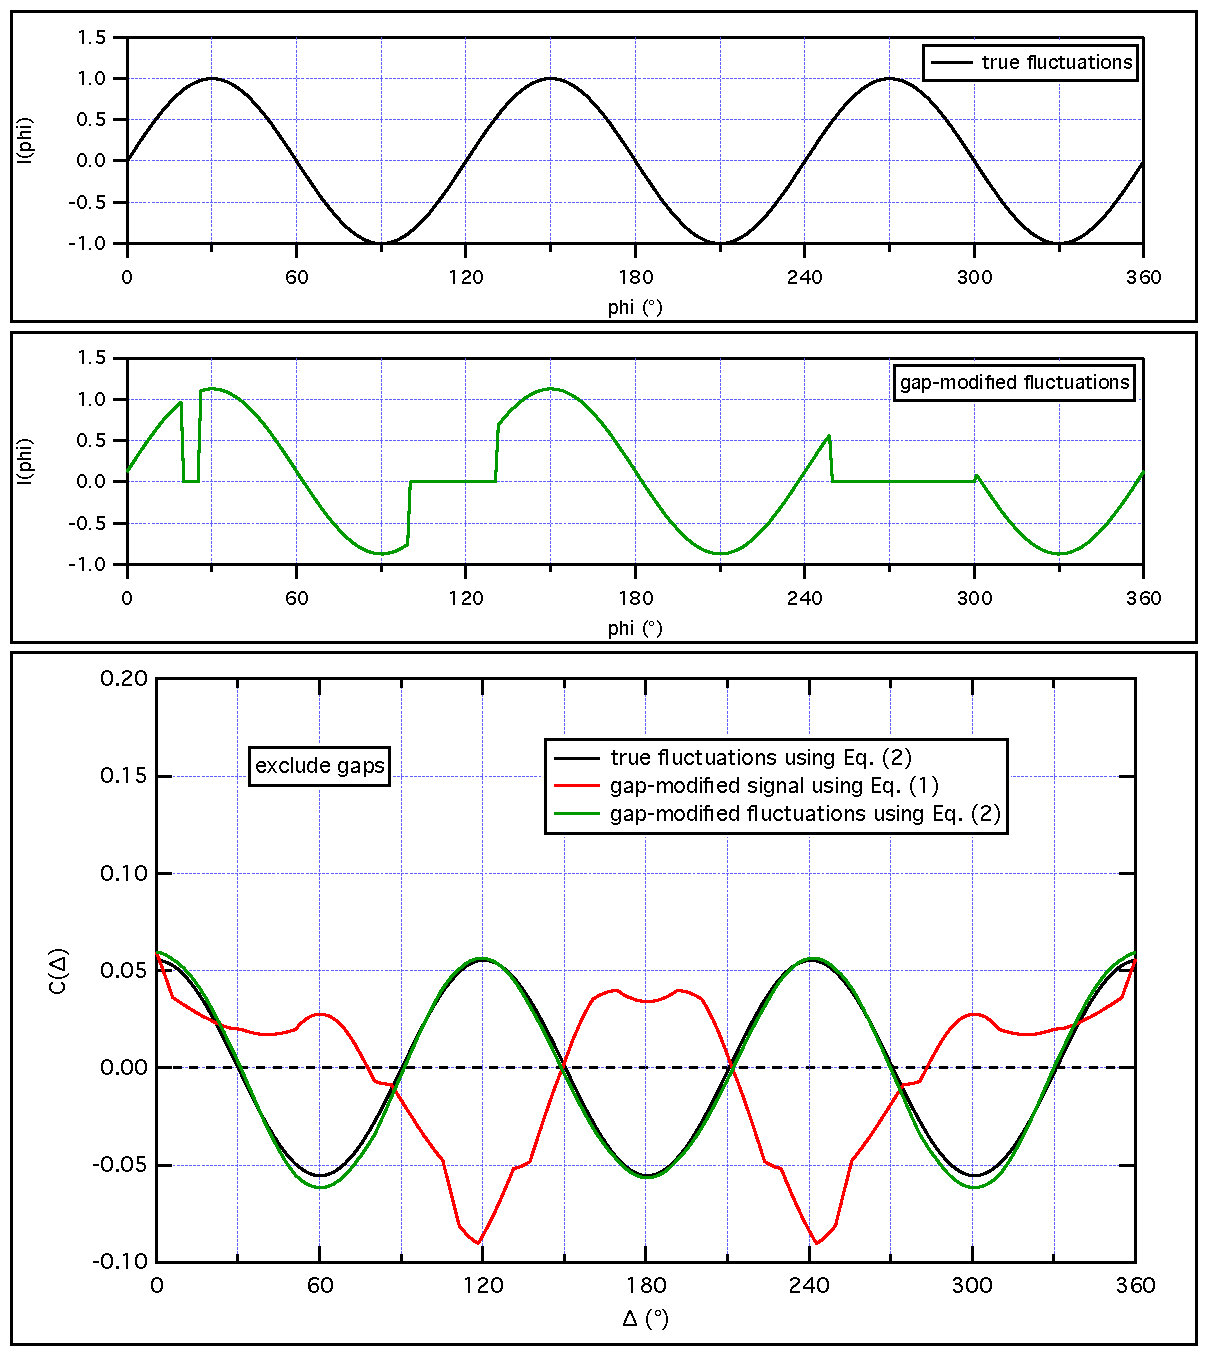
\includegraphics{./Layout1-exclude_gaps.pdf}}
  \caption{ \small (TOP) Model fluctuations of the scattered intensity at arbitrary $q$ with an angular dependence of sine function with a period of $2\pi/3$ that has an amplitude of 1. (MIDDLE) Gap-modified fluctuations where the presence of arbitrarily placed gaps modify the angular dependence of the scattered intensity by replacing the true signal by zeros. (BOTTOM) $C(\Delta)$ from correlating while excluding the gaps for the true signal using Eq. (\ref{xcca-int}) (black curve), the gap-modified signal using Eq. (\ref{xcca-int}) (red curve), and the gap-modified fluctuations using Eq. (\ref{xcca-fluct}) (green curve).}
  \label{fig-exclude-gaps}
\end{figure}

\begin{figure}
  \centering
  \scalebox{0.9}{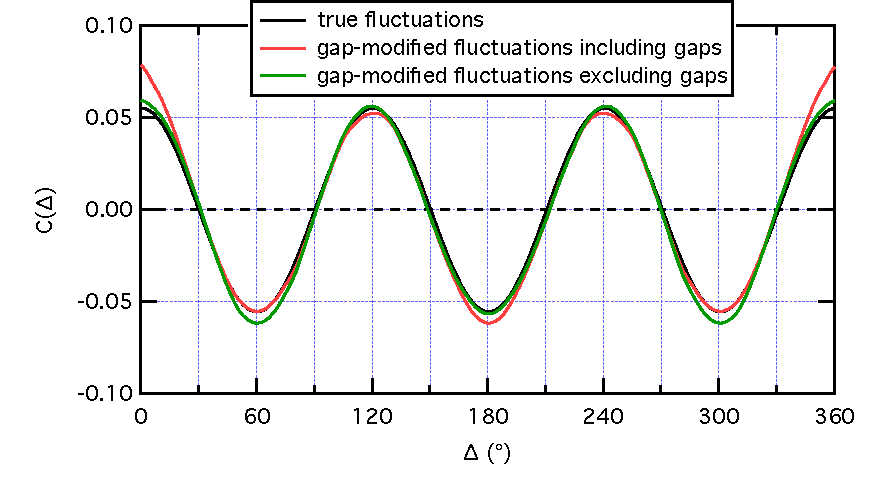
\includegraphics{./Graph13-eq2.pdf}}
  \caption{ \small $C(\Delta)$ calculated using Eq. (\ref{xcca-fluct}) for the true signal, the gap-modified fluctuations including the gaps (red curve), and the gap-modified fluctuations excluding the gaps (green curve).}
  \label{fig-xcca-fluct}
\end{figure}

\end{document}